% ********** Rozdział 4 **********
\chapter{Harmonogram realizacji projektu}

{W tym rozdziale przedstawiony jest harmonogram realizacji projektu aplikacji muzycznej, "Music Player", opracowanej w języku C\#. Harmonogram ten jest graficznie reprezentowany za pomocą diagramu Gantta: }

\begin{figure}[!ht]
	\begin{center}
	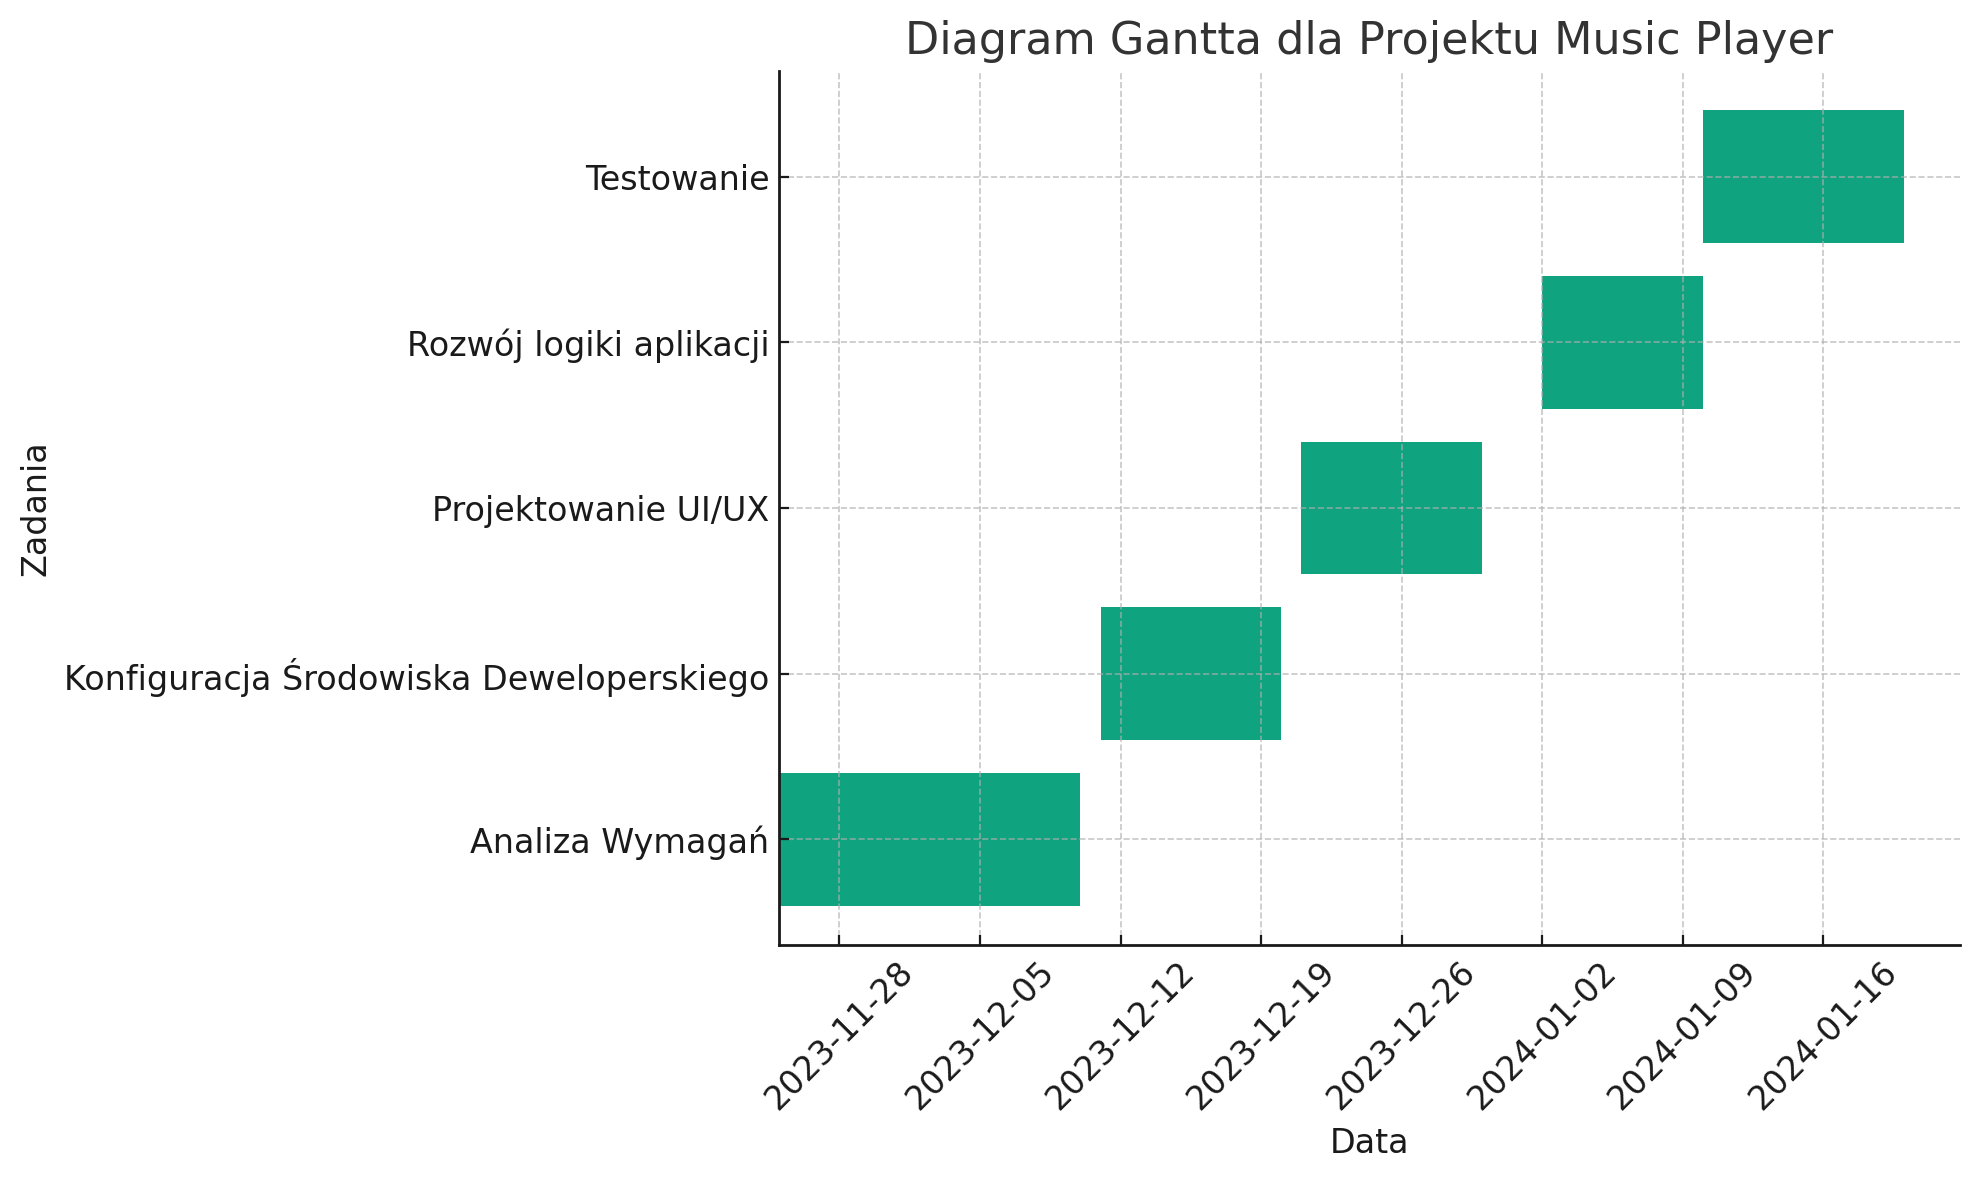
\includegraphics[height=200pt]{figures/diagram_gantta.png}
        \caption{{\footnotesize Schema bazy danych}}
	\end{center}
\end{figure}

{Szczegółowy opis zadań dla projektu:}

\begin{enumerate}
    \item \textbf{ Analiza Wymagań} (25.11.2023 - 10.12.2023)
    
        Czas na zrozumienie i zebranie kluczowych funkcjonalności wymaganych przez aplikację. Proces ten obejmuje przygotowanie listy narzędzi potrzebnych do wykonania projektu, analizę konkurencyjnych aplikacji. Jest to fundament, na którym opiera się cały projekt.
    \item \textbf{ Konfiguracja Środowiska Deweloperskiego} (11.12.2023 - 20.12.2023) 
    
    Ustanowienie odpowiedniego środowiska deweloperskiego jest kluczowe dla produktywności. W tym okresie zostało skonfigurowane IDE, zależności, docker, docker-compose, biblioteki oraz repozytorium Git, aby zapewnić płynny start i ciągłość prac nad projektem.
    \item \textbf{ Projektowanie UI/UX:} (21.12.2023 - 30.12.2023)
    
        Projekt interfejsu użytkownika (UI) oraz doświadczenia użytkownika (UX) ma bezpośredni wpływ na odbiór aplikacji przez użytkowników. W tym czasie budowany był cały główny interfejs UI by już na gotowej bazie okodować cała logikę aplikacji.
        \newpage

    \item \textbf{ Rozwój logiki aplikacji:} (02.1.2024 - 09.1.2024)

        Kluczowy etap rozwoju projektu, gdzie fokus położony był na implementację zaprojektowanego interfejsu użytkownika z właściwymi mechanizmami działania aplikacji. Ten okres pracy obejmował kodowanie głównych funkcji aplikacji, takich jak odtwarzanie muzyki, zarządzanie playlistami.
    \item \textbf{ Testowanie }  (10.01.2024 - 20.01.2024)
    
    Testowanie jest niezbędnym etapem w cyklu życia oprogramowania. W tym okresie aplikacja była testowana manualnie i poprawiana na bieżąco. W testowaniu pomagał również wcześniej stworzony skrypt CI/CD, który przy każdym zatwierdzeniu zmian automatycznie sprawdzał, czy aplikacja kompiluje się poprawnie.
    
\end{enumerate}

\section{Repozytorium i System Kontroli Wersji}

{Projekt jest rozwijany z użyciem systemu kontroli wersji Git, co pozwala na efektywną współpracę i śledzenie historii zmian. Repozytorium projektu znajduje się na GitHub pod adresem: \newline
\textbf{https://github.com/byko-dev/music-player}. Projekt będzie zamieszczony pod danym linkiem do dnia 31.03.2025. Dzięki wykorzystaniu Git, możliwe było efektywne zarządzanie kodem źródłowym.}

\section{Problemy i Trudności}
{W trakcie realizacji projektu Music Player napotkano różnorodne wyzwania. Jednym z nich było zapewnienie wysokiej jakości interfejsu użytkownika, co wymagało dokładnego planowania i testowania. Największym wyzwaniem okazało się stworzenie systemu do importu i eksportu danych z aplikacji. Zaplanowane wcześniej relacje w tabelach nie ułatwiały zadania, ponieważ program eksportował niechciane i często błędne dane, a podczas importu trudno było zachować relacje między tabelami. Dosyć szybko okazało się konieczne odejście od importu/eksportu tabeli Files, ponieważ była to operacja wymagająca i zasobożerna. Rozwiązaniem problemu okazało się stworzenie obiektów z prefixem 'Raw', które nie implementują relacji tabelarycznych.
}